% --- Conteúdo FINAL para Tabela&Grafico/comparativo_geral.tex ---

\qquad A etapa final do trabalho consiste na análise comparativa do desempenho dos cinco algoritmos estudados: \textit{Bubble Sort}, \textit{Insertion Sort}, \textit{Selection Sort}, \textit{Shell Sort} e \textit{Merge Sort}. Para facilitar a interpretação, os resultados foram organizados por cenário de entrada, cada um com sua tabela de tempos e seu gráfico correspondente. Em todas as figuras, cada algoritmo é identificado por uma cor própria, mantida ao longo de toda a seção.

\qquad Os gráficos utilizam escala linear no eixo vertical, mantendo o mesmo padrão das figuras individuais de cada algoritmo. Como os tempos medidos variam de milésimos de segundo a mais de uma hora, as curvas dos algoritmos mais rápidos (\textit{Shell Sort} e \textit{Merge Sort}, além do \textit{Insertion Sort} no cenário crescente) aparecem rentes ao eixo horizontal. Isso não indica ausência de dados, e sim valores pequenos demais para serem distinguidos em uma escala que precisa acomodar milhares de segundos. Os valores exatos podem ser consultados nas tabelas que acompanham cada gráfico.

\qquad Os nomes dados aos cenários (melhor, pior e médio caso) se referem ao comportamento dos algoritmos quadráticos e do \textit{Shell Sort}, cujo desempenho depende da ordem inicial dos dados. No caso do \textit{Merge Sort}, esses nomes indicam apenas o tipo de entrada utilizada, pois o algoritmo executa o mesmo trabalho em qualquer ordem.

\subsubsection*{Análise Comparativa por Cenário}

\paragraph{Cenário Crescente (Melhor Caso)}
A Figura \ref{fig:tabela_comp_melhor} e a Figura \ref{fig:grafico_comp_melhor} mostram o desempenho dos algoritmos com um vetor já ordenado. É neste cenário que se observa a maior diferença entre eles. O \textbf{Insertion Sort} levou apenas 0,005 segundo para um milhão de elementos, resultado que reflete sua complexidade $O(n)$ no melhor caso: com o vetor ordenado, a condição do laço interno falha na primeira verificação e nenhum deslocamento é realizado. O \textbf{Shell Sort} levou 0,099 segundo, também beneficiado pela ordenação prévia. O \textbf{Merge Sort} levou 0,155 segundo: ele não tira proveito da ordenação, pois executa todas as divisões e intercalações mesmo com o vetor ordenado, mas seu custo $O(n \log n)$ já é baixo o bastante para ficar próximo dos dois anteriores. Em contraste, o \textbf{Bubble Sort} (1.474,120s) e o \textbf{Selection Sort} (1.365,660s) mantiveram comportamento quadrático, pois nenhuma das duas implementações possui mecanismo capaz de detectar que o vetor já está ordenado e interromper a execução.

\begin{figure}[!htb]
    \centering
    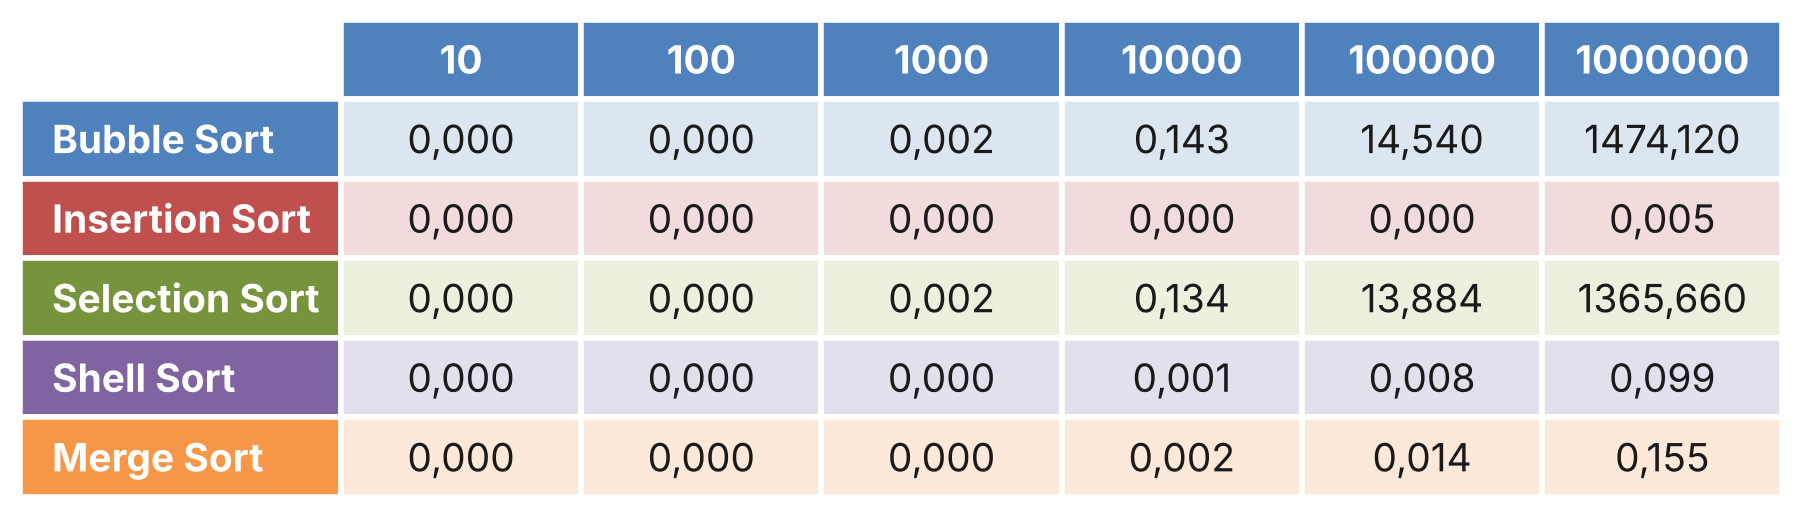
\includegraphics[width=0.8\textwidth]{Imagens/Geral/tabela_comp_melhorcaso.png}
    \caption{Tempos de execução (em segundos) dos cinco algoritmos - Cenário Crescente (elaborado pelo autor).}
    \label{fig:tabela_comp_melhor}

    \vspace{0.5cm}

    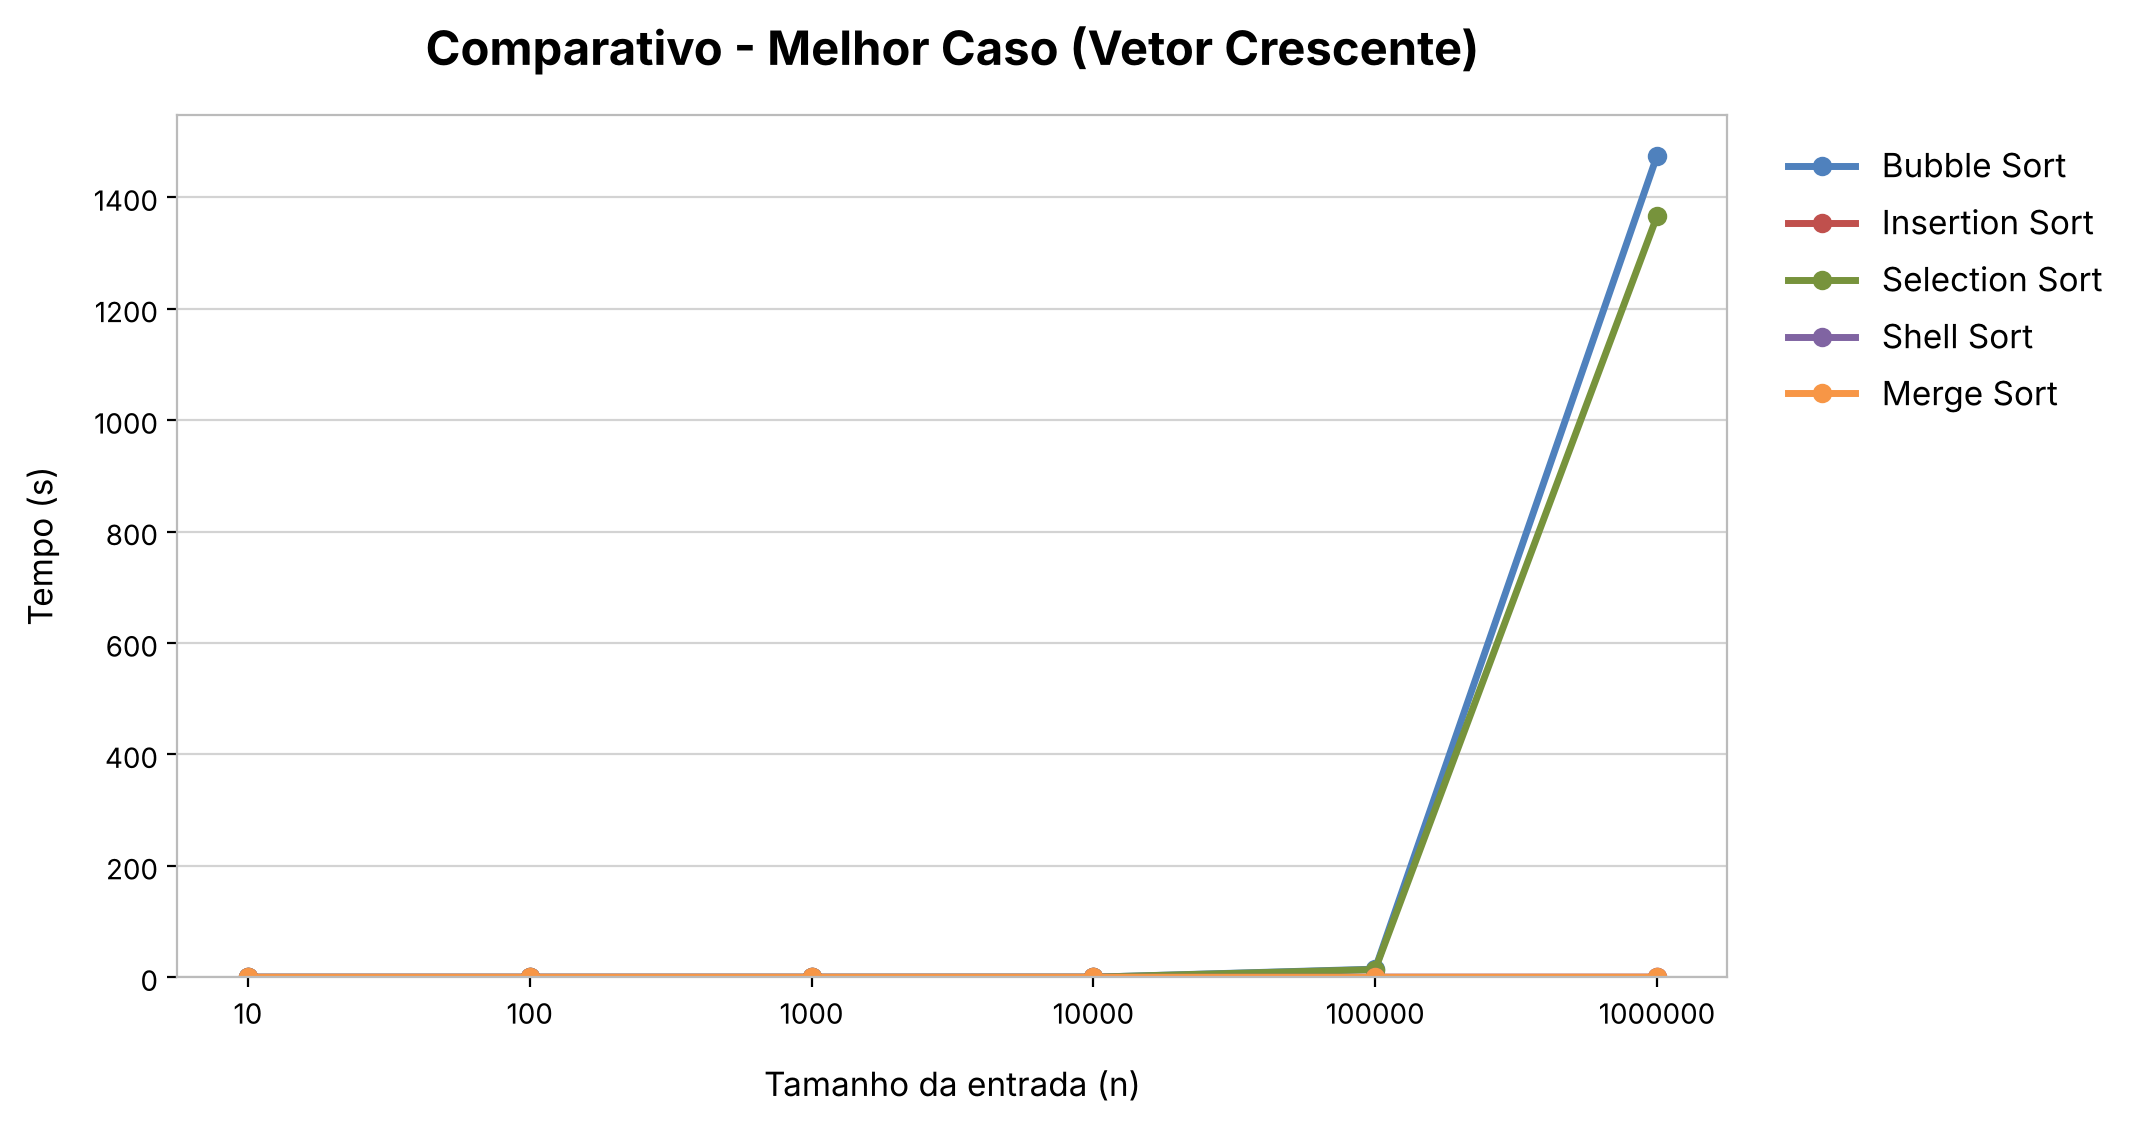
\includegraphics[width=0.8\textwidth]{Imagens/Geral/grafico_comp_melhorcaso.png}
    \caption{Comparativo de Desempenho dos Algoritmos - Cenário Crescente (elaborado pelo autor).}
    \label{fig:grafico_comp_melhor}
\end{figure}

\FloatBarrier

\paragraph{Cenário Decrescente (Pior Caso)}
Com os dados em ordem inversa, apresentados na Figura \ref{fig:tabela_comp_pior} e na Figura \ref{fig:grafico_comp_pior}, os algoritmos quadráticos são os mais exigidos. O \textbf{Shell Sort} (0,129 segundo) e o \textbf{Merge Sort} (0,168 segundo) permanecem ordens de grandeza mais rápidos, com tempos muito próximos entre si. O tempo do \textit{Merge Sort} neste cenário é praticamente o mesmo do cenário crescente (0,155s), o que confirma que seu desempenho não depende da ordem dos dados. Entre os quadráticos, o \textbf{Bubble Sort} apresenta o pior desempenho absoluto, com 3.913,080s (aproximadamente 1h05min), por realizar uma troca a cada comparação efetuada. O \textbf{Insertion Sort} (2.164,840s) e o \textbf{Selection Sort} (1.561,630s) também se mostram impraticáveis nesta escala, com vantagem para o \textit{Selection Sort}, que se limita a $n-1$ trocas no total, independentemente da ordem inicial dos dados.

\begin{figure}[!htb]
    \centering
    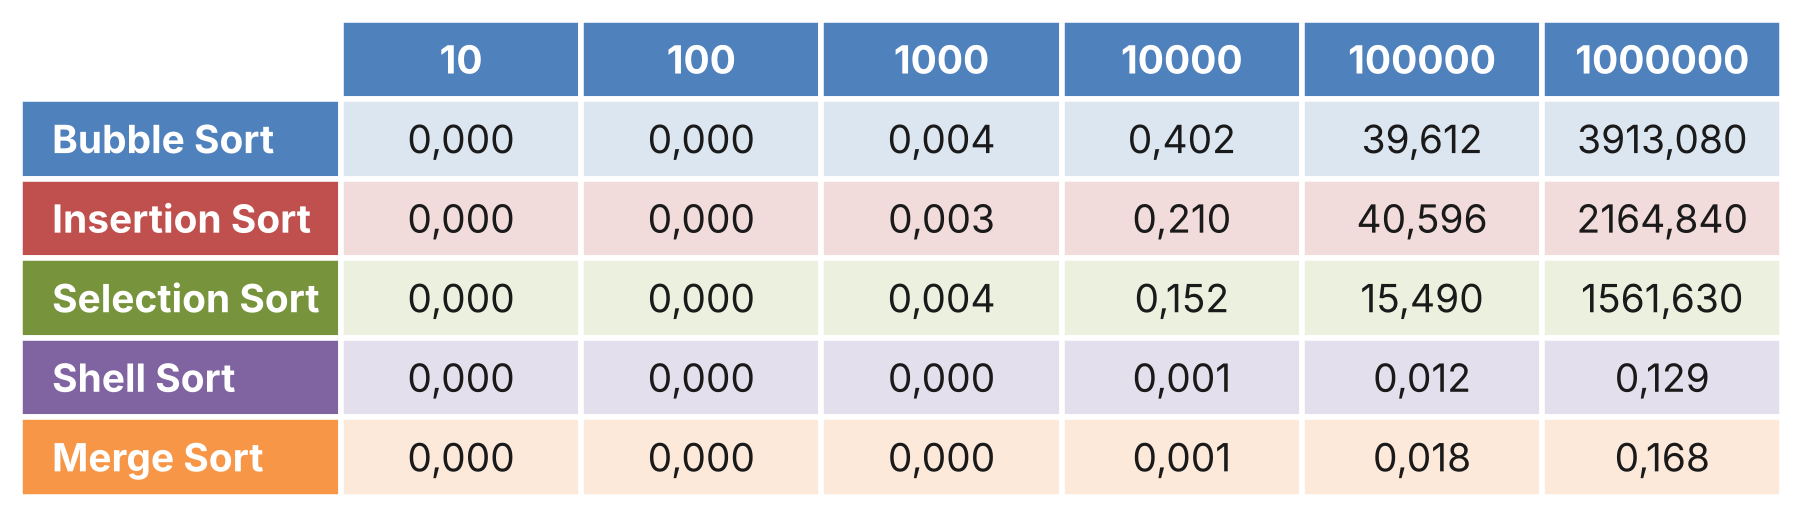
\includegraphics[width=0.8\textwidth]{Imagens/Geral/tabela_comp_piorcaso.png}
    \caption{Tempos de execução (em segundos) dos cinco algoritmos - Cenário Decrescente (elaborado pelo autor).}
    \label{fig:tabela_comp_pior}

    \vspace{0.5cm}

    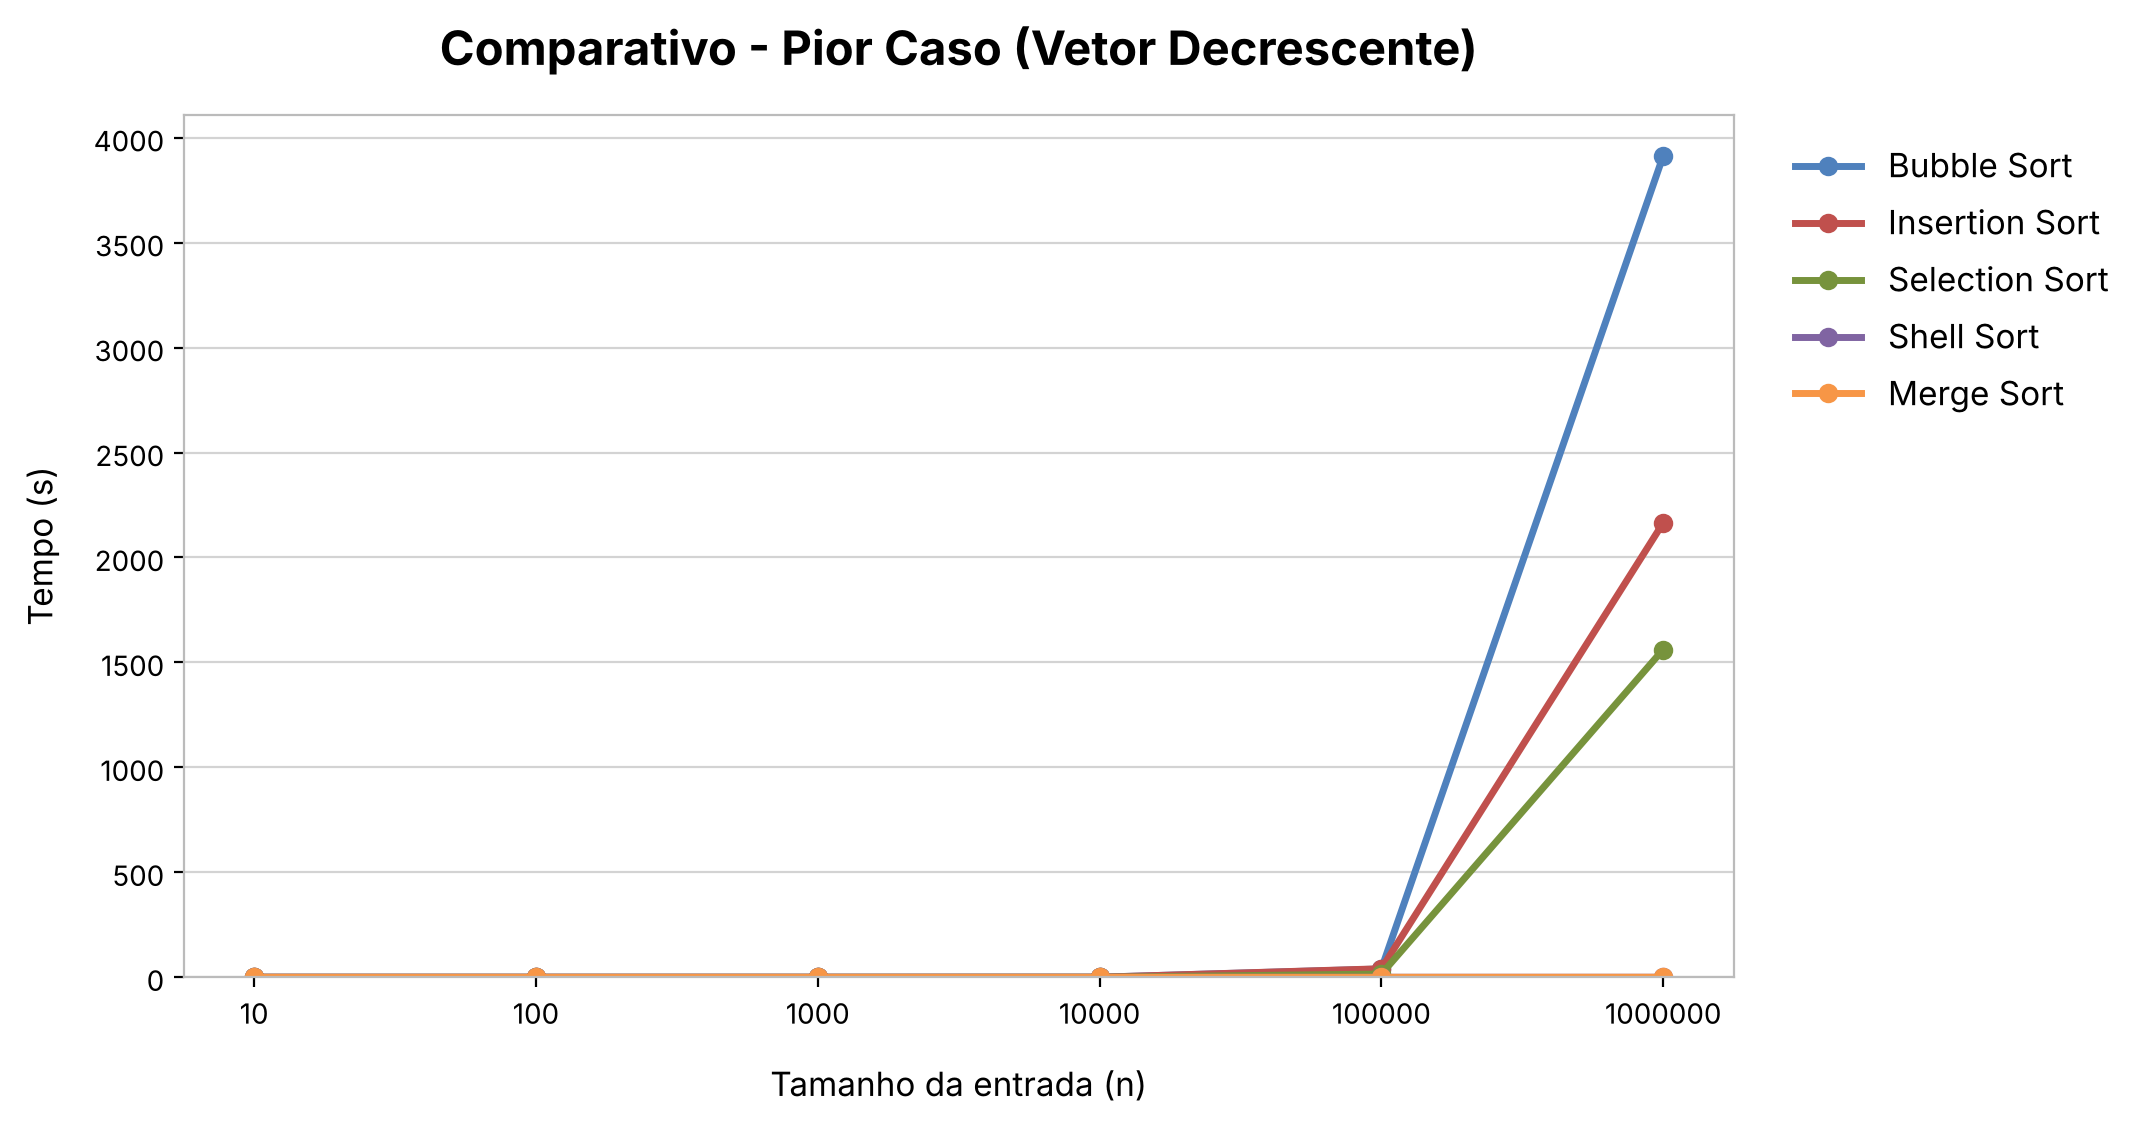
\includegraphics[width=0.8\textwidth]{Imagens/Geral/grafico_comp_piorcaso.png}
    \caption{Comparativo de Desempenho dos Algoritmos - Cenário Decrescente (elaborado pelo autor).}
    \label{fig:grafico_comp_pior}
\end{figure}

\FloatBarrier

\paragraph{Cenário Randômico (Caso Médio)}
A Figura \ref{fig:tabela_comp_medio} e a Figura \ref{fig:grafico_comp_medio} representam o cenário de uso mais comum e consolidam as observações anteriores. O \textbf{Merge Sort} se firma como a escolha superior, com apenas 0,292 segundo, seguido pelo \textbf{Shell Sort}, com 0,461 segundo. Este é o único cenário em que o \textit{Merge Sort} supera o \textit{Shell Sort}, pois o \textit{Shell Sort} depende da ordem dos dados e perde parte da vantagem quando eles estão desordenados. No grupo dos quadráticos, o \textbf{Insertion Sort} (1.086,290s) é o mais rápido, seguido pelo \textbf{Selection Sort} (1.658,270s) e, por último, pelo \textbf{Bubble Sort} (3.954,730s). O tempo do \textit{Insertion Sort} corresponde a aproximadamente metade do registrado em seu pior caso, comportamento coerente com a expectativa teórica de que, em média, cada elemento percorre metade da distância até sua posição final. Comparados ao \textit{Merge Sort}, o \textit{Insertion Sort} foi cerca de 3.700 vezes mais lento, o \textit{Selection Sort} cerca de 5.700 vezes e o \textit{Bubble Sort} cerca de 13.500 vezes.

\begin{figure}[!htb]
    \centering
    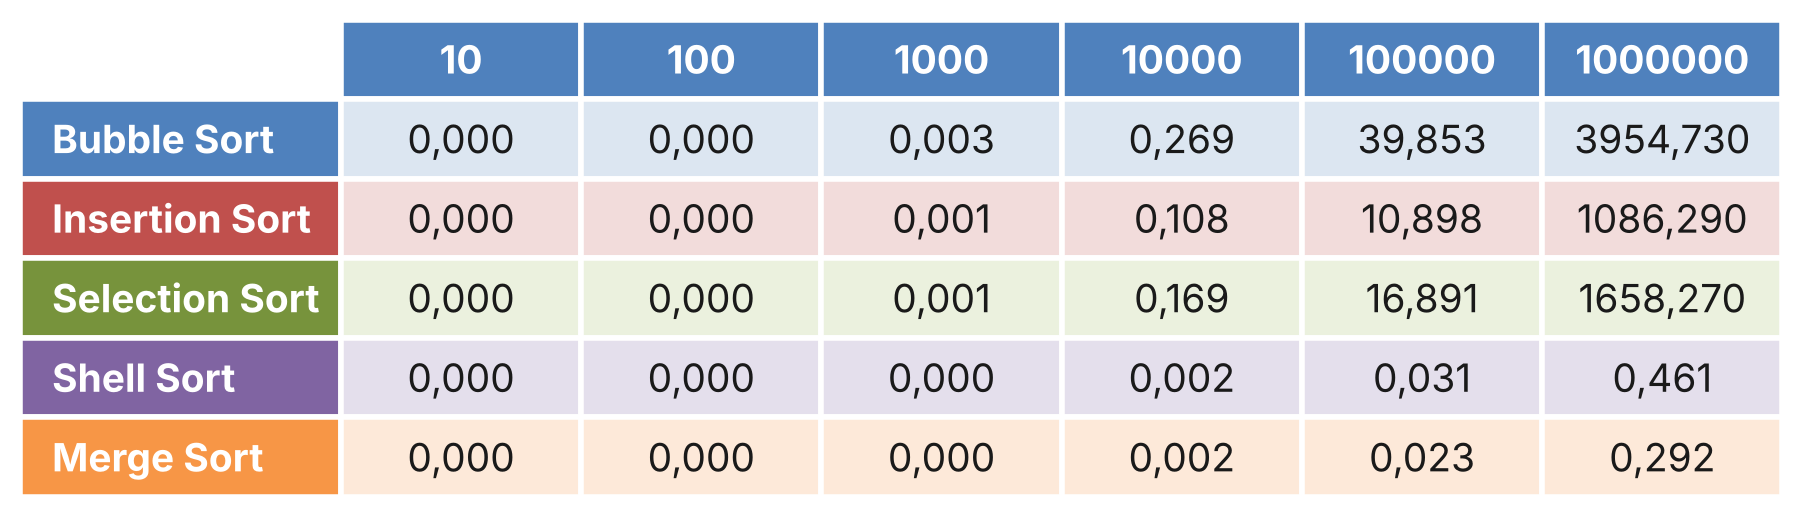
\includegraphics[width=0.8\textwidth]{Imagens/Geral/tabela_comp_casomedio.png}
    \caption{Tempos de execução (em segundos) dos cinco algoritmos - Cenário Randômico (elaborado pelo autor).}
    \label{fig:tabela_comp_medio}

    \vspace{0.5cm}

    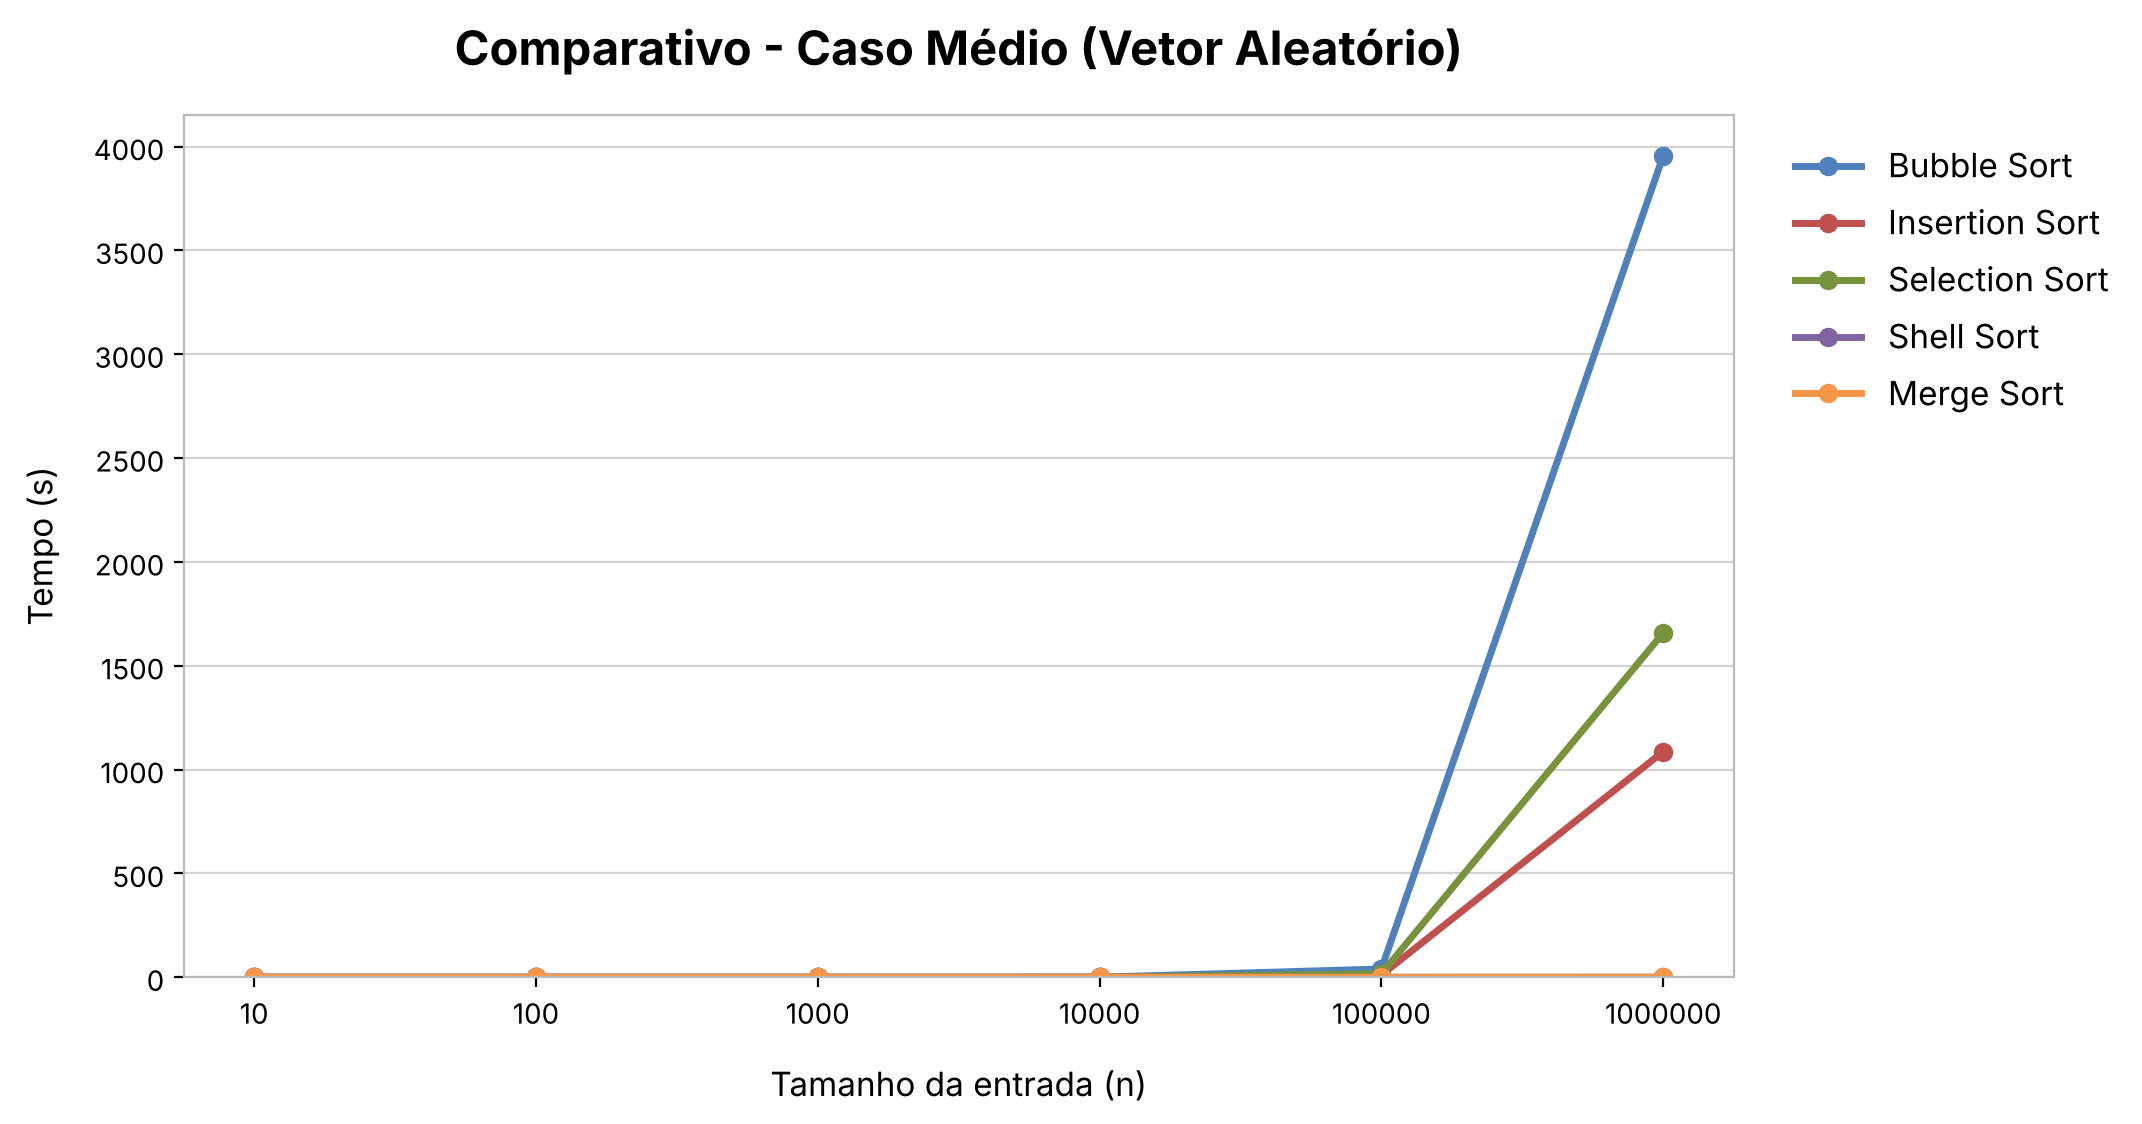
\includegraphics[width=0.8\textwidth]{Imagens/Geral/grafico_comp_casomedio.png}
    \caption{Comparativo de Desempenho dos Algoritmos - Cenário Randômico (elaborado pelo autor).}
    \label{fig:grafico_comp_medio}
\end{figure}

\FloatBarrier

\subsubsection*{Síntese da Análise Comparativa}

\qquad A análise conjunta dos três cenários permite dividir os algoritmos em duas categorias de desempenho. Os de complexidade $O(n^2)$ (\textit{Bubble}, \textit{Insertion} e \textit{Selection}) são adequados apenas para fins didáticos ou para entradas pequenas, tendo levado mais de vinte minutos para ordenar um milhão de elementos na maioria dos cenários. O \textit{Shell Sort}, com complexidade subquadrática, e o \textit{Merge Sort}, com complexidade $O(n \log n)$ em todos os casos, concluíram a mesma tarefa em menos de meio segundo em qualquer cenário.

\qquad Entre os quadráticos, cada um apresenta uma característica distinta. O \textit{Insertion Sort} é o mais sensível à ordem da entrada, variando de 0,005s a 2.164,840s entre o melhor e o pior caso, o que o torna a melhor opção quando há expectativa de dados parcialmente ordenados. O \textit{Selection Sort} é o mais previsível, com variação de apenas 21\% entre os cenários, sendo preferível quando o custo de cada troca é elevado. O \textit{Bubble Sort} não apresentou vantagem em nenhum cenário, tendo sido o mais lento nas entradas decrescente e aleatória.

\qquad Entre os dois algoritmos mais rápidos, a escolha depende do tipo de entrada e dos recursos disponíveis. O \textit{Shell Sort} foi mais rápido nos cenários crescente e decrescente, pois aproveita a ordem prévia dos dados, e funciona \textit{in-place}, sem memória adicional. O \textit{Merge Sort} foi o mais rápido no cenário aleatório e manteve desempenho regular, variando de 0,155s a 0,292s entre os cenários, mas exige um vetor auxiliar de tamanho $n$. Além disso, é estável, o que o torna preferível quando se deseja preservar a ordem relativa de elementos iguais.

\qquad Vale registrar que, para entradas de até 1.000 elementos, os cinco algoritmos concluíram a ordenação em menos de 0,005 segundo, tornando a escolha irrelevante nessa faixa. A diferença entre eles só se torna determinante a partir de dezenas de milhares de elementos, o que reforça a importância de considerar a escala do problema ao selecionar um algoritmo de ordenação.

\FloatBarrier